\documentclass[preprint, 12pt, authoryear]{elsarticle}

\usepackage{amsmath}
\usepackage{amssymb}
\usepackage{aas_macros}
\usepackage{rotating}
\usepackage{xspace}
\usepackage{booktabs}
\usepackage{multirow}
\usepackage{color}
\usepackage{listings}
\usepackage{caption}
\usepackage{url}
\usepackage{adjustbox}
\journal{Astronomy and Computing}

%%% Definitions added by Manodeep 
\newcommand{\Msun}{M_{\odot}}
\newcommand{\hMsun}{h^{-1}M_{\odot}}
\newcommand{\sdss}{{\small{SDSS}}\xspace}
\newcommand{\hMpc}{\ensuremath{{h^{-1}Mpc}\xspace}}
\newcommand{\hkpc}{\ensuremath{{h^{-1}kpc}\xspace}}
\newcommand{\emcee}{\texttt emcee}
\newcommand{\corrfunc}{{\tt Corrfunc}\xspace}
\newcommand{\rmax}{\ensuremath{{{\mathcal{R}}_{max}}}\xspace}
\newcommand{\rmaxcubed}{\ensuremath{{\mathcal{R}^{3}_{max}}}\xspace}
\newcommand{\rsep}{\ensuremath{{{\mathcal{R}}_{sep}}}\xspace}
\newcommand{\lbox}{\ensuremath{\mathcal{L}}\xspace}
\newcommand{\npart}{\ensuremath{\mathcal{N}}\xspace}
\newcommand{\xir}{\ensuremath{{DD(r)}}\xspace}
\newcommand{\xiofr}{\ensuremath{{\xi(r)}}\xspace}
\newcommand{\wprp}{\ensuremath{{w_p(r_p)}}\xspace}
\newcommand{\xirppi}{\ensuremath{{\xi(r_p,\pi)}}\xspace}
\newcommand{\cis}{\ensuremath{{pN(r)}}\xspace}
\newcommand{\ddrppi}{\ensuremath{{DD(r_p,\pi)}}\xspace}
\newcommand{\wtheta}{\ensuremath{{DD(\theta)}}\xspace}
\newcommand{\todo}[1]{\marginpar{TODO}{\color{red}#1}}
\newcommand{\avx}{\texttt AVX}
\newcommand{\sse}{\texttt SSE}


\lstset{
  language=C,                % choose the language of the code
  basicstyle=\ttfamily,      % sets font
  numbers=left,                   % where to put the line-numbers
  numberstyle=\small, 
  stepnumber=1,                   % the step between two line-numbers.
  numbersep=10pt,                  % how far the line-numbers are from the code
  backgroundcolor=\color{white},  % choose the background color. You must add \usepackage{color}
  showspaces=false,               % show spaces adding particular underscores
  showstringspaces=false,         % underline spaces within strings
  showtabs=false,                 % show tabs within strings adding particular underscores
  tabsize=2,                      % sets default tabsize to 2 spaces
  captionpos=b,                   % sets the caption-position to bottom
  breaklines=true,                % sets automatic line breaking
  breakatwhitespace=true,         % sets if automatic breaks should only happen at whitespace
}

\begin{document}

\begin{frontmatter}

\title{Cache is King: Presenting \corrfunc -- a Suite of Fast Correlation Function Codes}

\author[ms]{Manodeep Sinha}
\ead{manodeep.sinha@vanderbilt.edu}
\address[ms]{6902 Stevenson Center, Department of Physics \& Astronomy, Vanderbilt University, Nashville, TN 37235}

\begin{abstract}
In the era of `Big Data', we need special computing techniques to both process the raw data as well 
generate and evaluate models to test our theories. In particular, large galaxy surveys
like the Sloan Digitial Sky Survey requires computing a variety of $n$-point statistics, e.g., the 
2-pt projected correlation function, $\wprp$. 
Since the clustering measure on the data is only done once, time taken to do
such a measurement is not a bottleneck. However, modeling the observed galaxy distribution correctly
{\em requires} a Monte-Carlo Markov Chain (MCMC) and repeated measurements of one or multiple
clustering statistics. In order to efficiently compute {\em any} clustering statistic,
we need to write code that is tuned for the underlying hardware. For
modern CPUs, such tuning involves proper utilization of the cache hierarchy {\em and}
vectorization with Single Instruction Multiple Data (SIMD) capable wide vector registers. 
In this paper, I present \corrfunc --  a suite of OpenMP parallelized, clustering
codes that exploit current CPU micro-architecture with hand-written Advanced
Vector Extensions (\avx) and  Streaming SIMD Extensions (\sse) intrinsics. 
Given a 3-D distribution of points in a cartesian system (i.e.,
generated from cosmological simulations), \corrfunc can compute spatial
3-D correlation functions \xir, \xiofr, \xirppi; 2-point 
projected correlation function \wprp; counts-in-spheres \cis. For a 3-D
particle distribution on the sky (i.e., mock galaxy catalogs, observed galaxies), the codes can compute 
projected correlation function \ddrppi, angular correlation function \wtheta as
well as \cis.  By design, \corrfunc is highly optimized 
and can compute \wprp for $\mathcal{O}$(1 million) galaxies in
$\sim 6$ seconds on a post-2011 CPU, which is a factor of few faster than 
existing public correlation function routines.  \corrfunc is
publicly available at \url{https://github.com/manodeep/Corrfunc/} while
benchmarks with existing codes are available at
\url{https://gist.github.com/manodeep/cffd9a5d77510e43ccf0}.
\end{abstract}

\begin{keyword}
methods: numerical \sep (cosmology:) large-scale structure of universe \sep
\end{keyword}

\end{frontmatter}

\section{INTRODUCTION}
The large-scale structure of the Universe can be now measured using $\mathcal{O}$(million) galaxies 
using data from current surveys like the Sloan Digitial Sky Survey (SDSS). Upcoming
surveys on the Large Synoptic Survey Telescope will probe even 
deeper and wider and aim to target on $\mathcal{O}$(10's of million) galaxies. With such a large galaxy data, 
we can measure the galaxy density field fairly accurately in the data. While the number of galaxies observed 
in these current and upcoming surveys is large, we have to compute the galaxy density fields {\em only once}. Thus, 
even a slow, correlation function code will be fine when measuring the data correlation function. 
However, predicting this galaxy  density field data will require an even larger number of model galaxies -- increasing the computational 
load of determining the density field even further. Typically, the modeling process also involves an MCMC -- 
requiring $\sim$ millions of evaluations of the correlation function.\footnote{I will assume that creating the models themselves 
is much faster compared to computing the correlation functions.} 

\section{BACKGROUND}
\subsection{HARDWARE ARCHITECTURE}
Modern cpu's have a hierarchy of memory locations; the smallest (and fastest) are physically located close to the computing cores 
while the largest (and slowest) are the farthest. All cpu instructions need to be carried out from cpu registers - there are $\sim 100$ 
registers typically available and the access times are essentially
instantaneous. Next up is the {\em L1} cache 
divided into {\em L1D} for data and {\em L1I} for instructions cache. Since 
the cpu always necessarily executes instructions that are close together, we will ignore the instruction cache from now on. Typical L1 cache 
sizes range from 64KB to 128 KB (shared between instruction and data). 
Next level up is the L2 cache, typically $\sim$ 256KB to 1 MB. The last level cache or the L3 cache is usually shared across all 
cores on the socket and can be 10 MB to 40 MB. 
\subsection{VECTORIZATION}

\subsection{OPTIMIZATION STRATEGIES}

\section{PACKAGE SUMMARY}
\corrfunc is written primarily in {\tt C} and comes with convenient
{\tt python} wrappers for typical clustering statistics. The fundamental design
principles for \corrfunc are the following:
\begin{enumerate}
  \item Correct -- \corrfunc has a base set of correct outputs for every statistic
    generated either through slow, brute-force methods or independent, 
    external codes. Within \corrfunc, every clustering statistic is covered with at least one
    test case that {\em requires} reproducing this `known-correct' result {\em
      exactly}. The `PASS/FAIL' status for each test is the direct output of {\tt diff -q
      test\_output known\_correct\_output}.  
  \item High Performance -- Performance is the overarching goal for {\tt
    Corrfunc}. The code-base has been repeatedly analyzed with Intel VTune
    (\url{https://software.intel.com/en-us/intel-vtune-amplifier-xe})
    on a variety of platforms to optimize the innermost loops. 
  \item Portable -- \corrfunc is written in {\tt ISO/IEC 9899:1999}
    compliant {\tt C}. All instruction set specific codes are protected via compile-time constant
    definitions.
\end{enumerate}
Every clustering statistic in \corrfunc can either be accessed through the
API call (e.g., via {\tt python}), linking with the static libraries) or as
a command-line executable. 

\section{Methods}
\subsection{Complexity of the Code}
We need to compute pairwise~\citep{} distances to get the correlation function. A naive implementation of a correlation function would compute {\em all possible} 
pairwise separations with a complexity $\mathcal{O}(N^2)$. However, for almost all correlation functions, we are only interested in separations less than 
a certain \rmax, where \rmax is much smaller than the domain of the point distribution itself. We can then immediately see a way to prune pairs that can not
{\em possibly} be within \rmax. If we impose a 3-d grid, with cell-size \rmax, then two points separated by more than one cell size (\rmax) in any one 
dimension can not be within \rmax of each other. Thus, given one point which is the target galaxy and a grid with cell-size \rmax, 
immediately allows us to prune {\em all} of the points that are not within 1 cell offset along each dimension. However, even with this pruning, the actual 
implementation of the algorithm matters. For instance, a linked-list in each cell performs $\sim 60\times$ worse than the algorithm described here.\footnote{The 
usual linked-list is very cache-unfriendly. Each dereference requires a read
from a new region of memory and an almost guaranteed cache miss. } 
We can now compute the theoretical complexity of the proposed algorithm. Let
\lbox be the side-length of the cube over which $\mathcal{N}$ points are distributed, then
each cell contains $r_{\mathrm max}^3\times \mathcal{N/V}$ particles. To compute the
correlation function, we have to loop over each point, and then {\em all} of
the points in the neighboring cells. This results in a complexity of 
$\mathcal{O(NM)}$, where $\mathcal{M} = \mathcal{N}\times\left(\rmax/\lbox\right)^3$. Typical \rmax is $\sim 0.10-0.2\times
\lbox$, therefore ordering the particles in cells of size \rmax should
result in a speedup of $(\rmax/\lbox)^3 \sim 125-1000$ compared to the
brute-force algorithm. Since every possible pair within \rmax has to be
examined, the algorithm deteriorates to $\mathcal{O(N}^2)$ for \rmax comparable
to \lbox. Space partitioning tree based approaches are far more suitable for
cases where \rmax is $\gtrsim 0.5\times\lbox$~\citep[e.g.,][]{mlpack2013,
  feng_kdcount}. 

\subsection{Partitioning the Particles based on \rmax}
Fig.~\ref{fig:grid} shows a schematic 2-D grid for the partitioning scheme. The
red circles represents the reference Poisson distributed points while the blue filled circle
shows the query point. The grid is constructed in the exact same way for both
datasets such that the 2-D (the index is in 3-D for the actual code)  index for the query point is identical to that of
the reference dataset. Once the central cell is determined, {\em any} reference
point that satisfies the distance inequality $\rsep < \rmax$, {\em must} lie
within the shaded 9 cells (corresponds to 27 in 3-D). 
\begin{figure}[htbp]
\centering
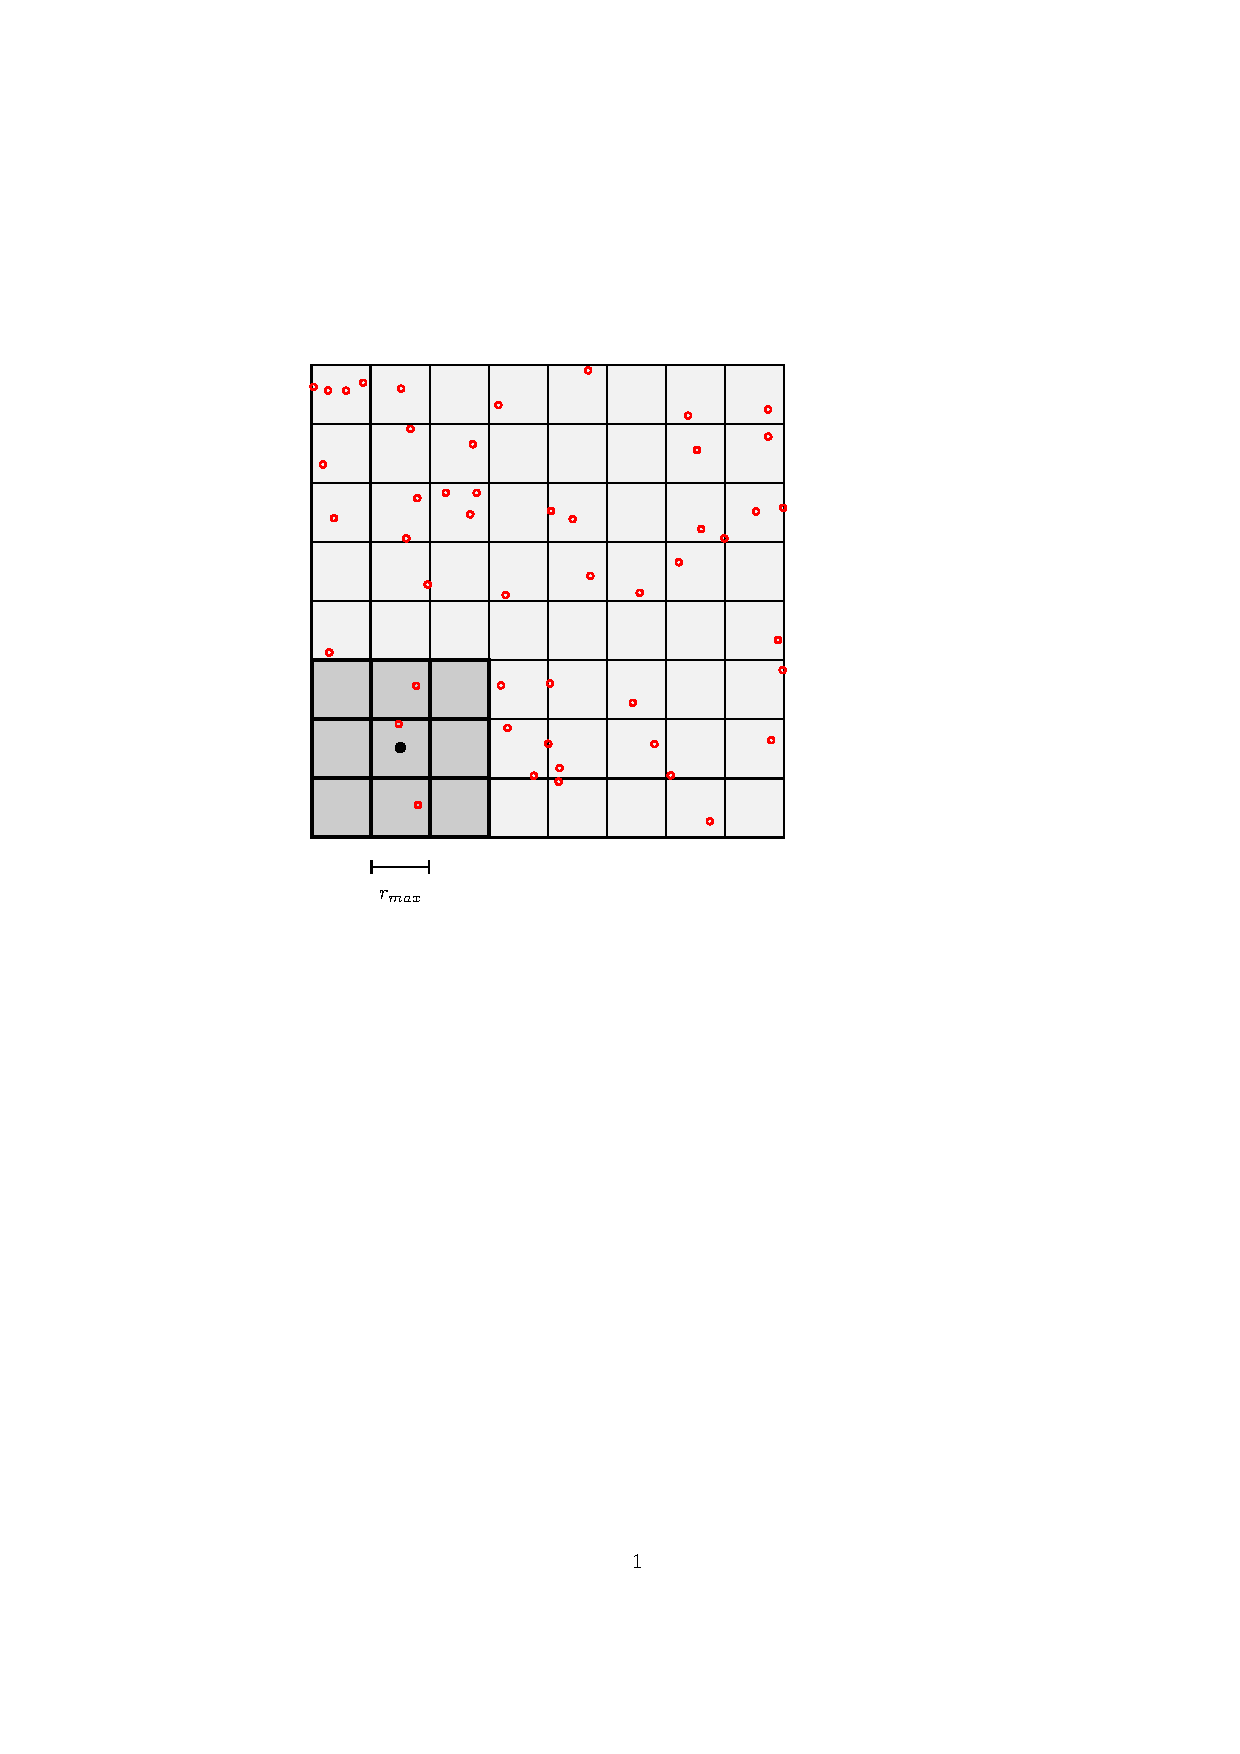
\includegraphics[clip=true]{tikz_grid}
\caption{A 2-D grid showing the bin-lattice partitioning scheme. The bigger square show the entire 
domain, the red circles show a random distribution of 100 particles. Let's say we want to compute all pairs 
for the target blue point, then we would only have to consider red points that are within one cell (the dark shaded region). 
A circle with radius \rmax is also drawn to shown the actual pairs that will eventually count in the correlation function.} 
\label{fig:grid}
\end{figure}


\subsection{How to Maintain Cache Locality within the Grid}
For all pairs around a given target galaxy, we need to compute distances to all points within all neighbouring 3-d cells. 
We ensure that the particle locations are contiguous by moving them into the following \texttt{C struct} in the order in which they arrive. 

\begin{lstlisting}
typedef struct{
  DOUBLE *x;
  DOUBLE *y;
  DOUBLE *z;
  int64_t nelements;
} cellarray;
\end{lstlisting}

Since the typical particle data is small ($\sim$ 20-30 MB), duplicating the entire particle distribution does not impose a strong 
constraint on the memory requirements. However, this duplication allows us to store the particles contiguously and produces fewer 
cache misses while looping over particles in a cell. 
The entire 3-D particle distribution is then deposited on the uniform grid. Now, for each particle we need to visit 27 total cells to 
compute all possible pairs within \rmax. 

\section{The pair-counting algorithm}

\subsection{\xir}
\subsection{\xirppi}
\subsection{\wprp}
\subsection{}

\subsection{Hand-written Vectorization Support}
Advanced Vector Extensions (AVX) has been available in cpu's more recent than 2011. AVX allows the processing of 8 floats or 4 double simultaneously -- thus, 
potentially increasing the throughput by a factor of 8x/4x. However, automatic vectorization is not always possible by the compiler and in those cases 
we can write AVX vector intrinsics to directly manipulate 8 floats/4 doubles\footnote{Another option would be to use the vectorclass written by Agner Fog here: \url{http://agner.org/optimize/vectorclass/}}. 

\section{Benchmarks \& Scaling}
In this section we present the runtimes and scalings for different number of particles, \rmax and OpenMP threads for the codes. 
For all of the scaling tests, only an auto-correlation calculation was used and the fiducial catalog contains $\sim 1.2$ million 
galaxies on a periodic cube of side 420 \hMpc. 

\subsection{Scaling with Number of Particles}
In Fig.~\ref{fig:scaling_numpart}, we show the scaling for the three codes with the number of particles. For this scaling, we subsampled 
the fiducial mock to attain 10 logarithmic steps in particle number ranging from $1.2\times10^4$ to $1.2\times10^6$. 

\begin{figure}[htbp]
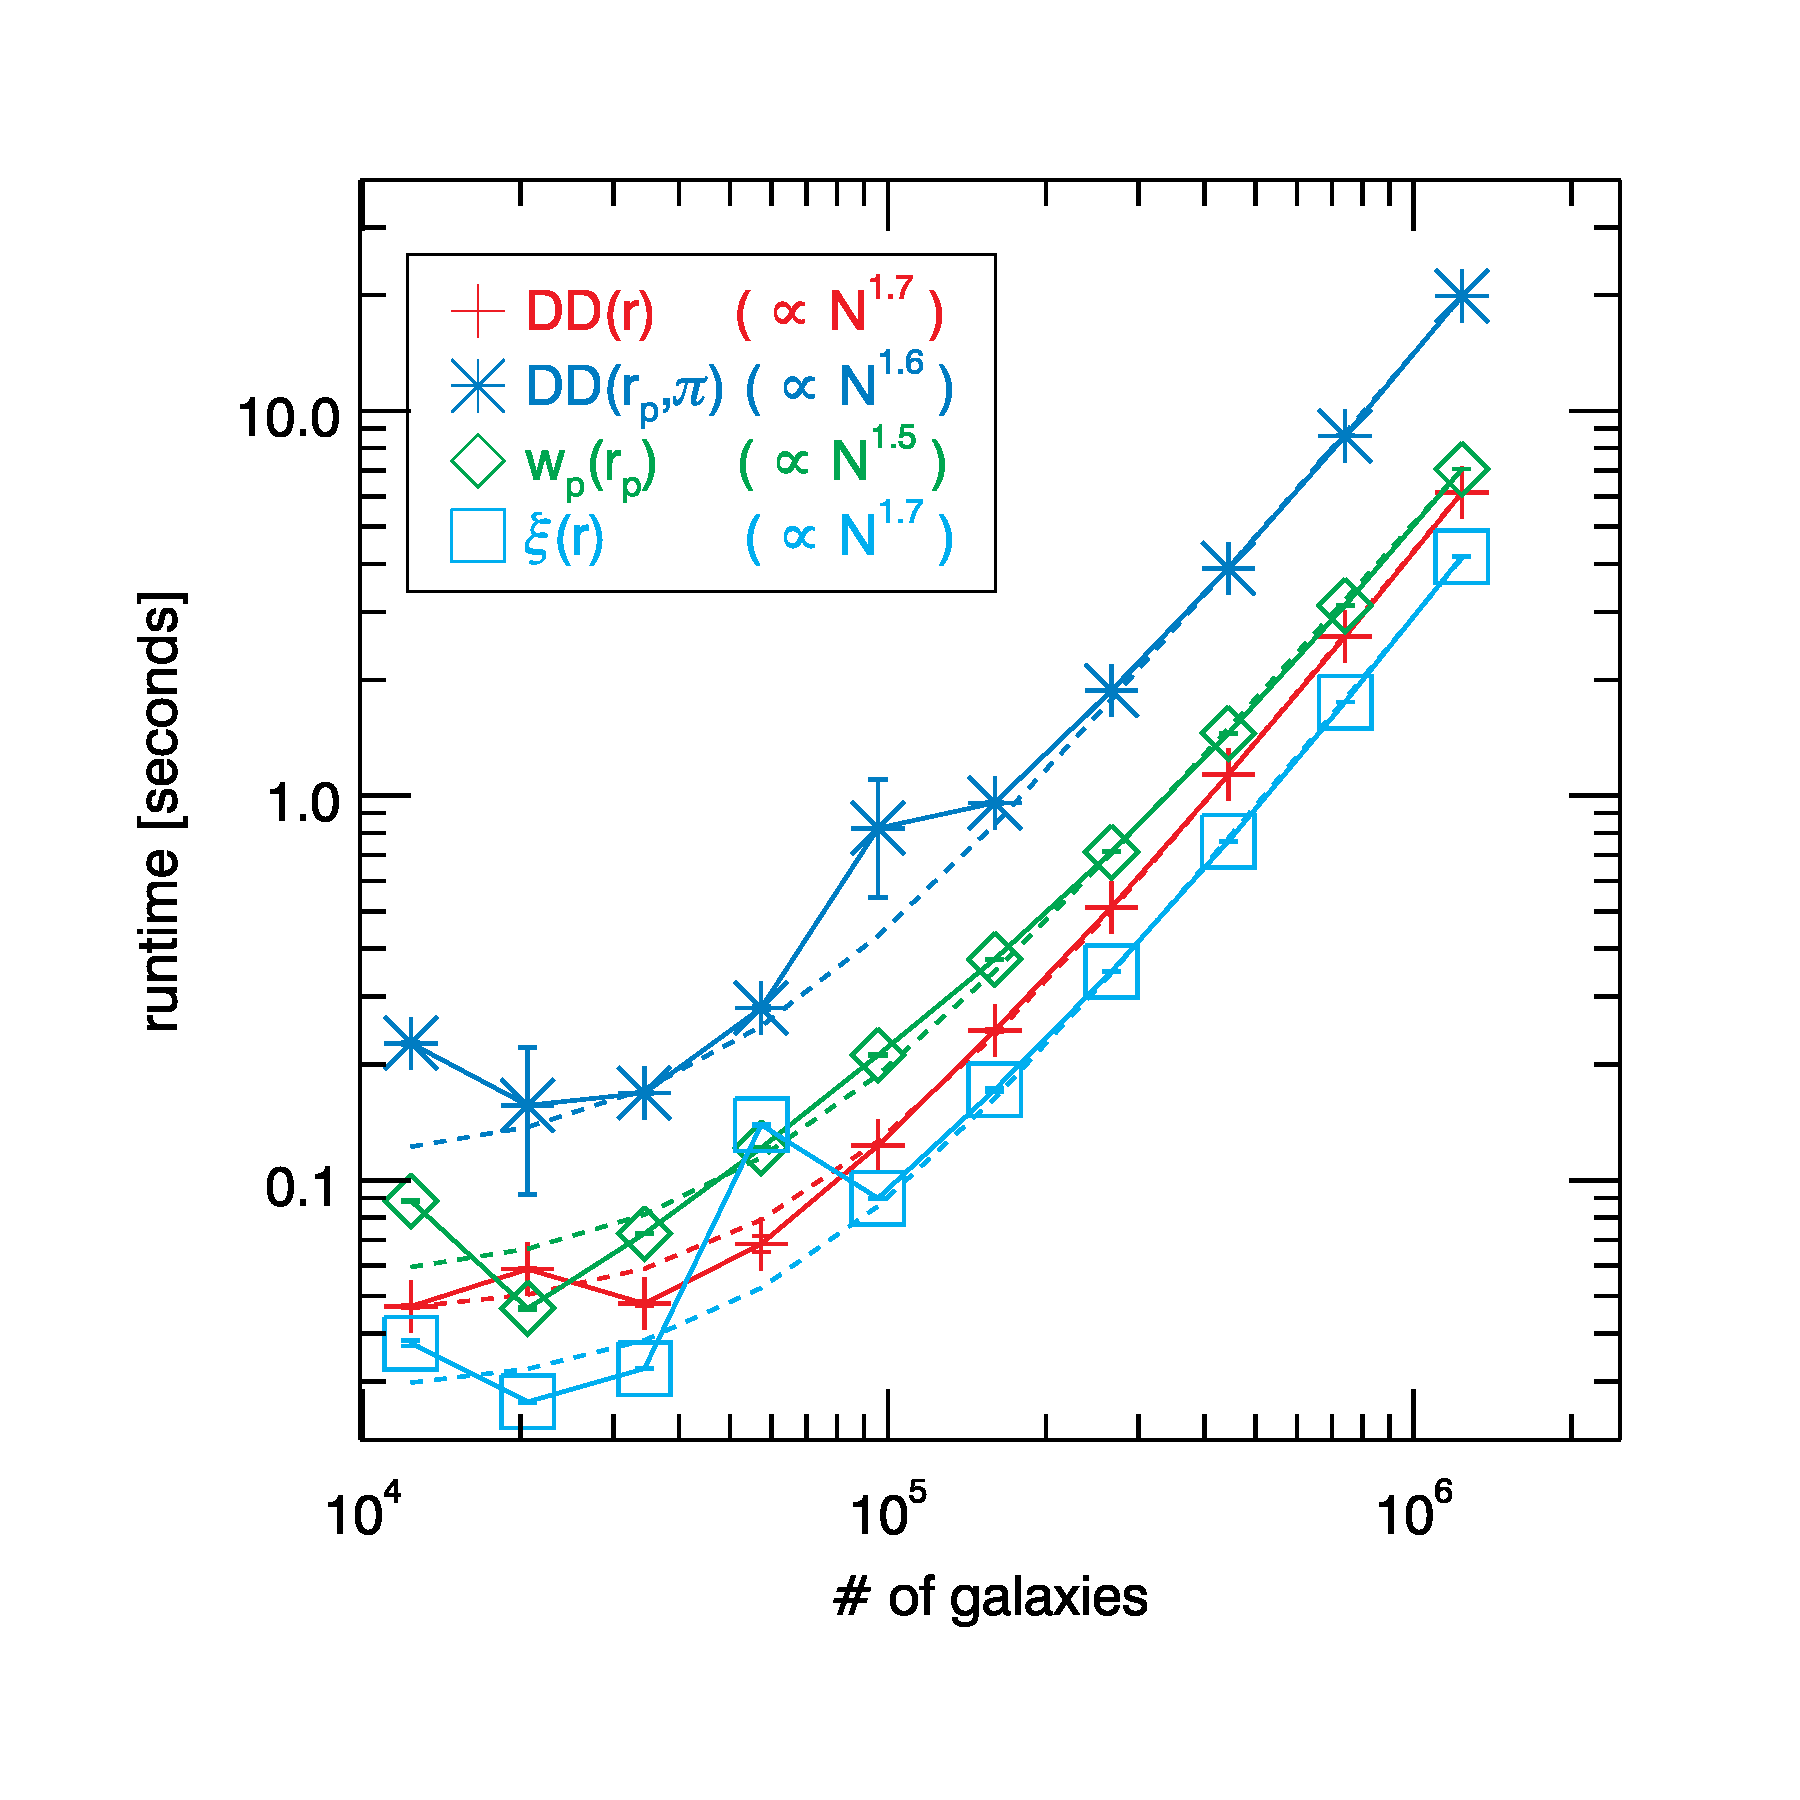
\includegraphics[clip=true,width=\linewidth]{timings_Mr19_numpart}%
\caption{Scaling with particle number for \xir, \xirppi, \wprp and \xiofr}
\label{fig:scaling_numpart}
\end{figure}

\subsection{Scaling with \rmax}
\begin{figure}[htbp]
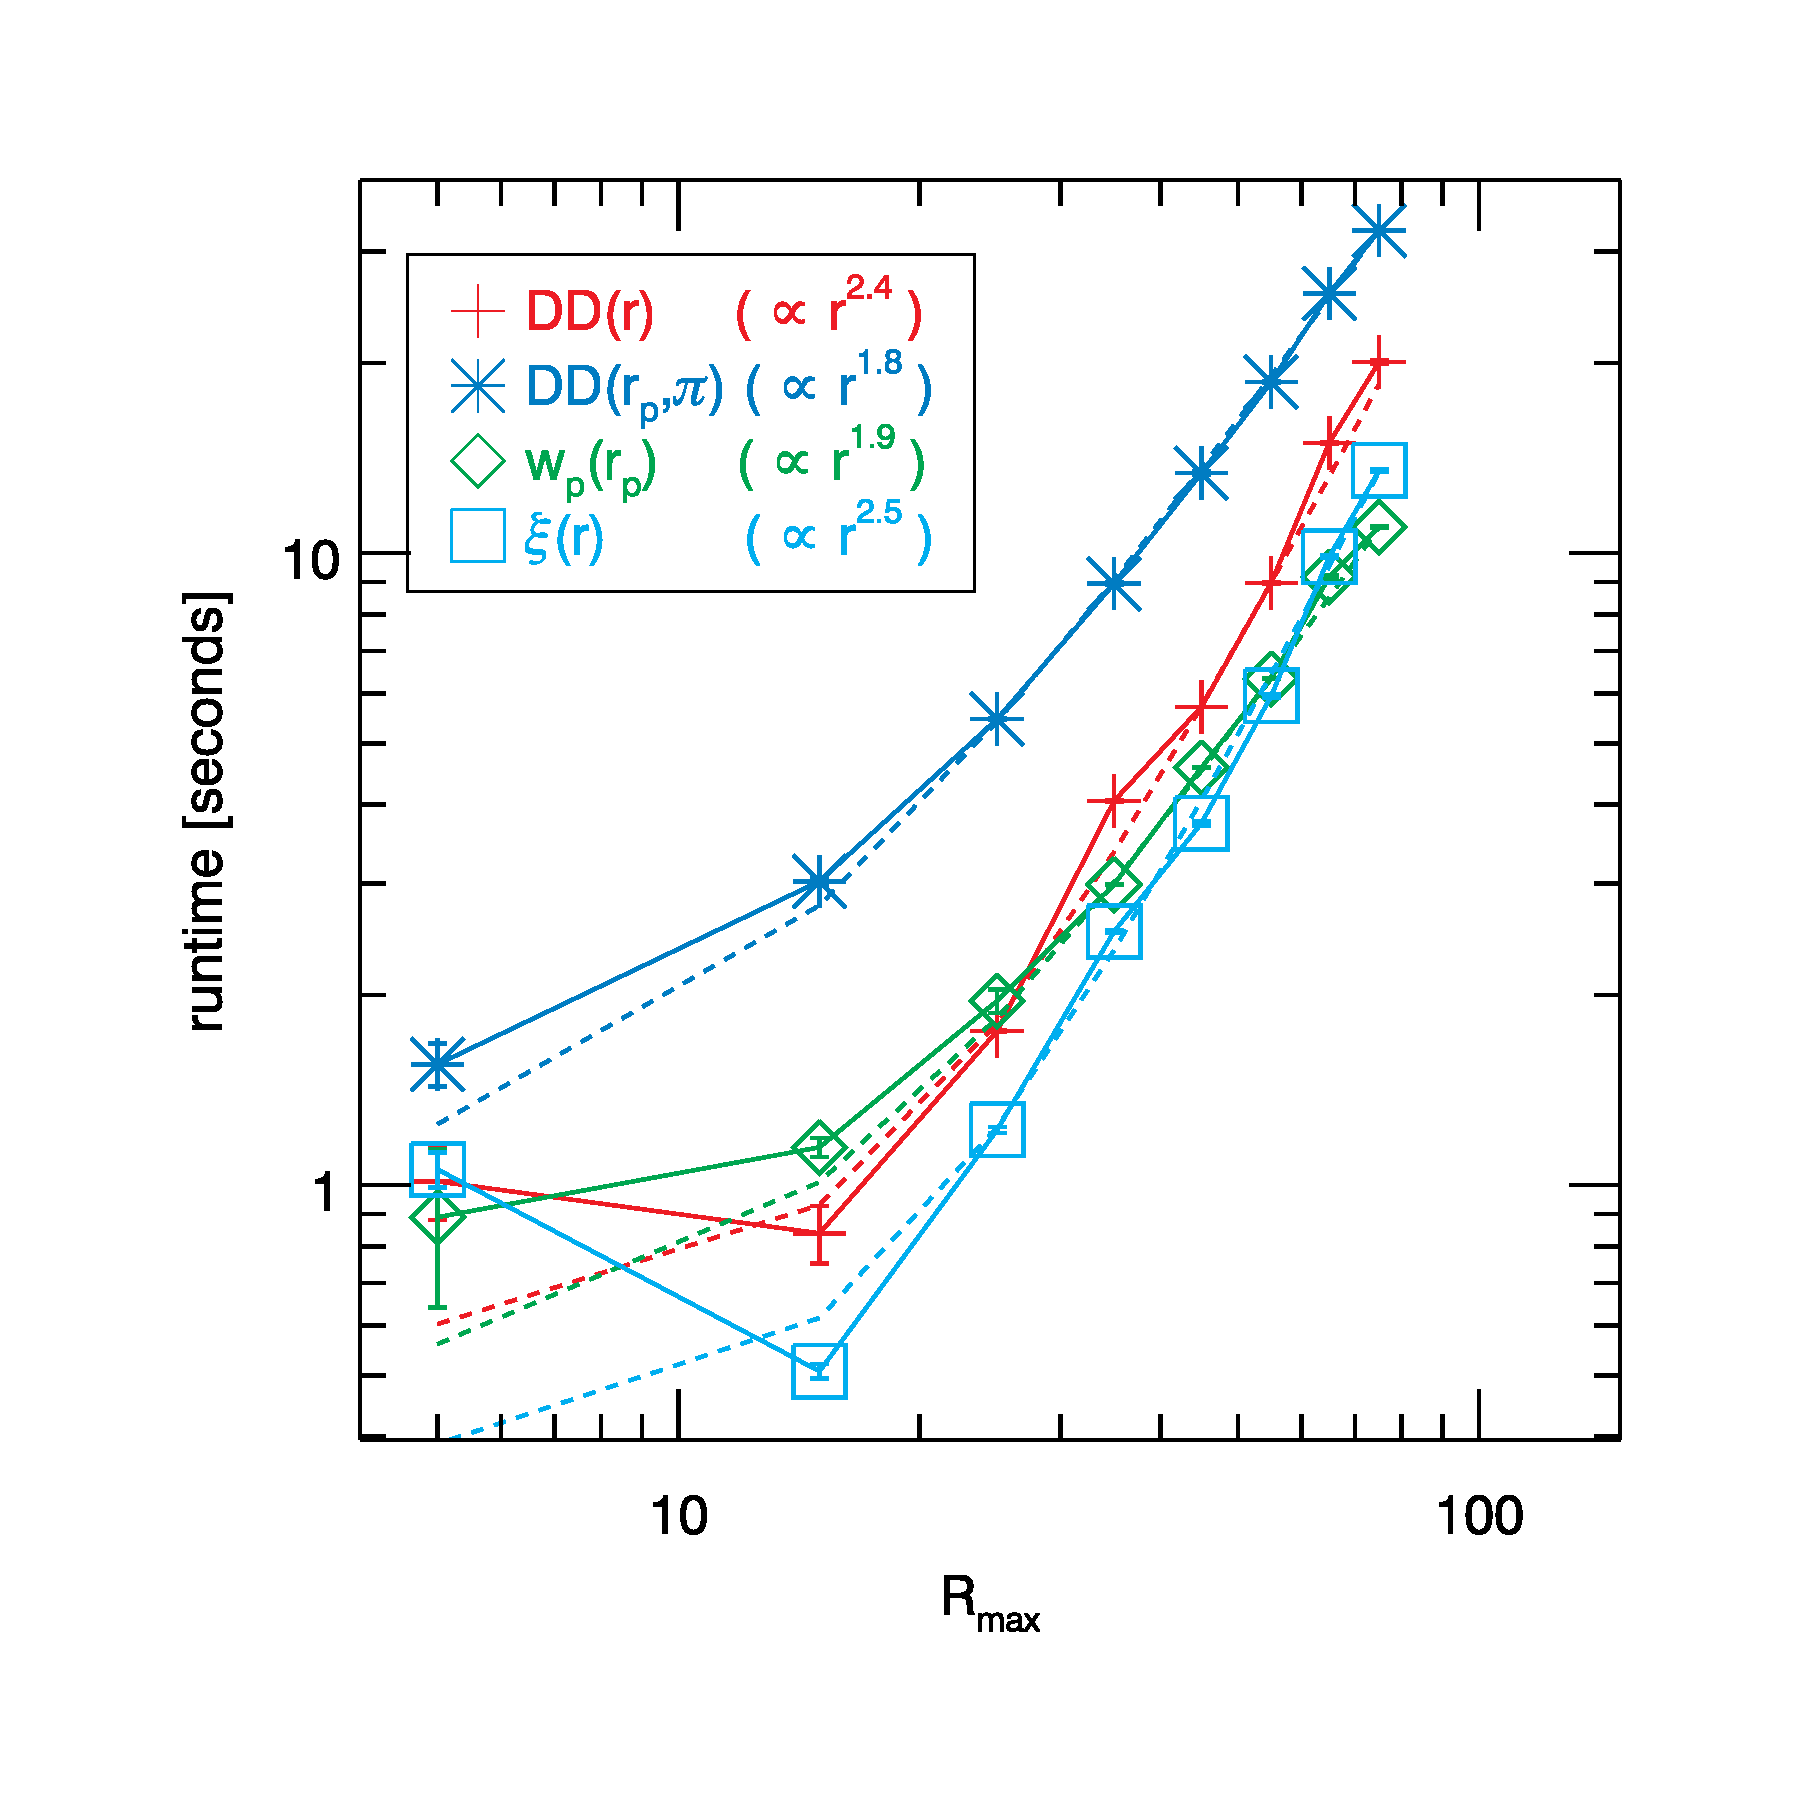
\includegraphics[clip=true,width=0.5\linewidth]{timings_Mr19_rmax}%
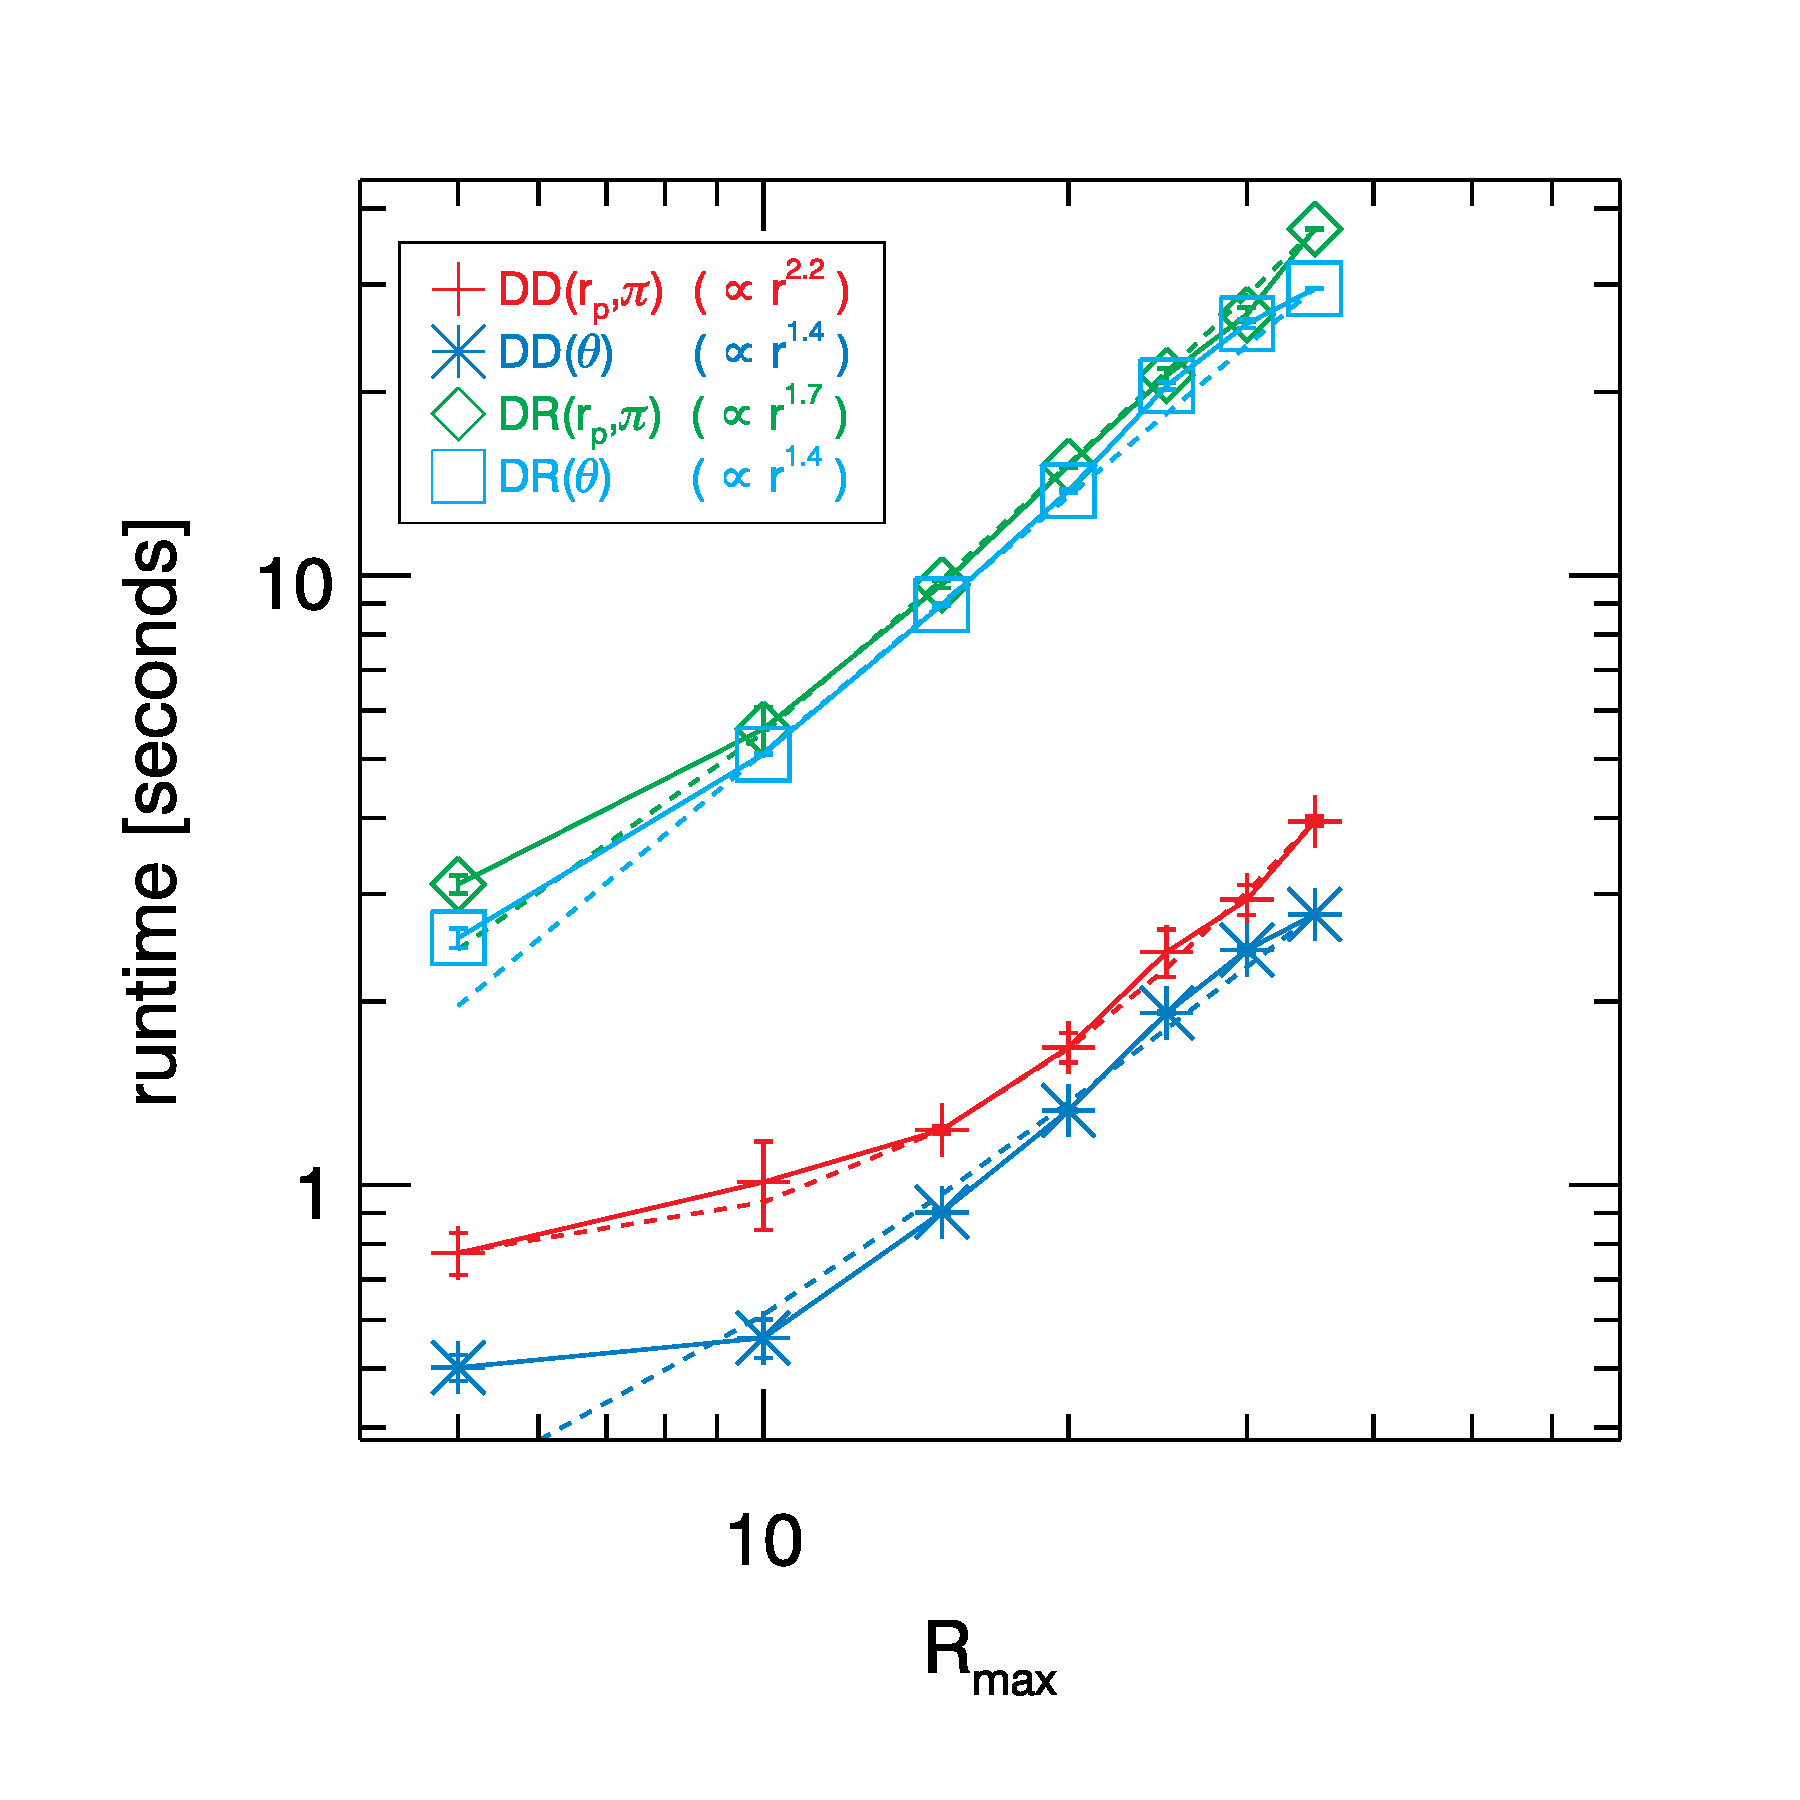
\includegraphics[clip=true,width=0.5\linewidth]{timings_Mr19_mocks_rmax}
\caption{Scaling with \rmax for \xir, \xirppi, \wprp and \xiofr}
\label{fig:scaling_rmax}
\end{figure}


\subsection{Scaling with OpenMP threads}
\begin{figure}[htbp]
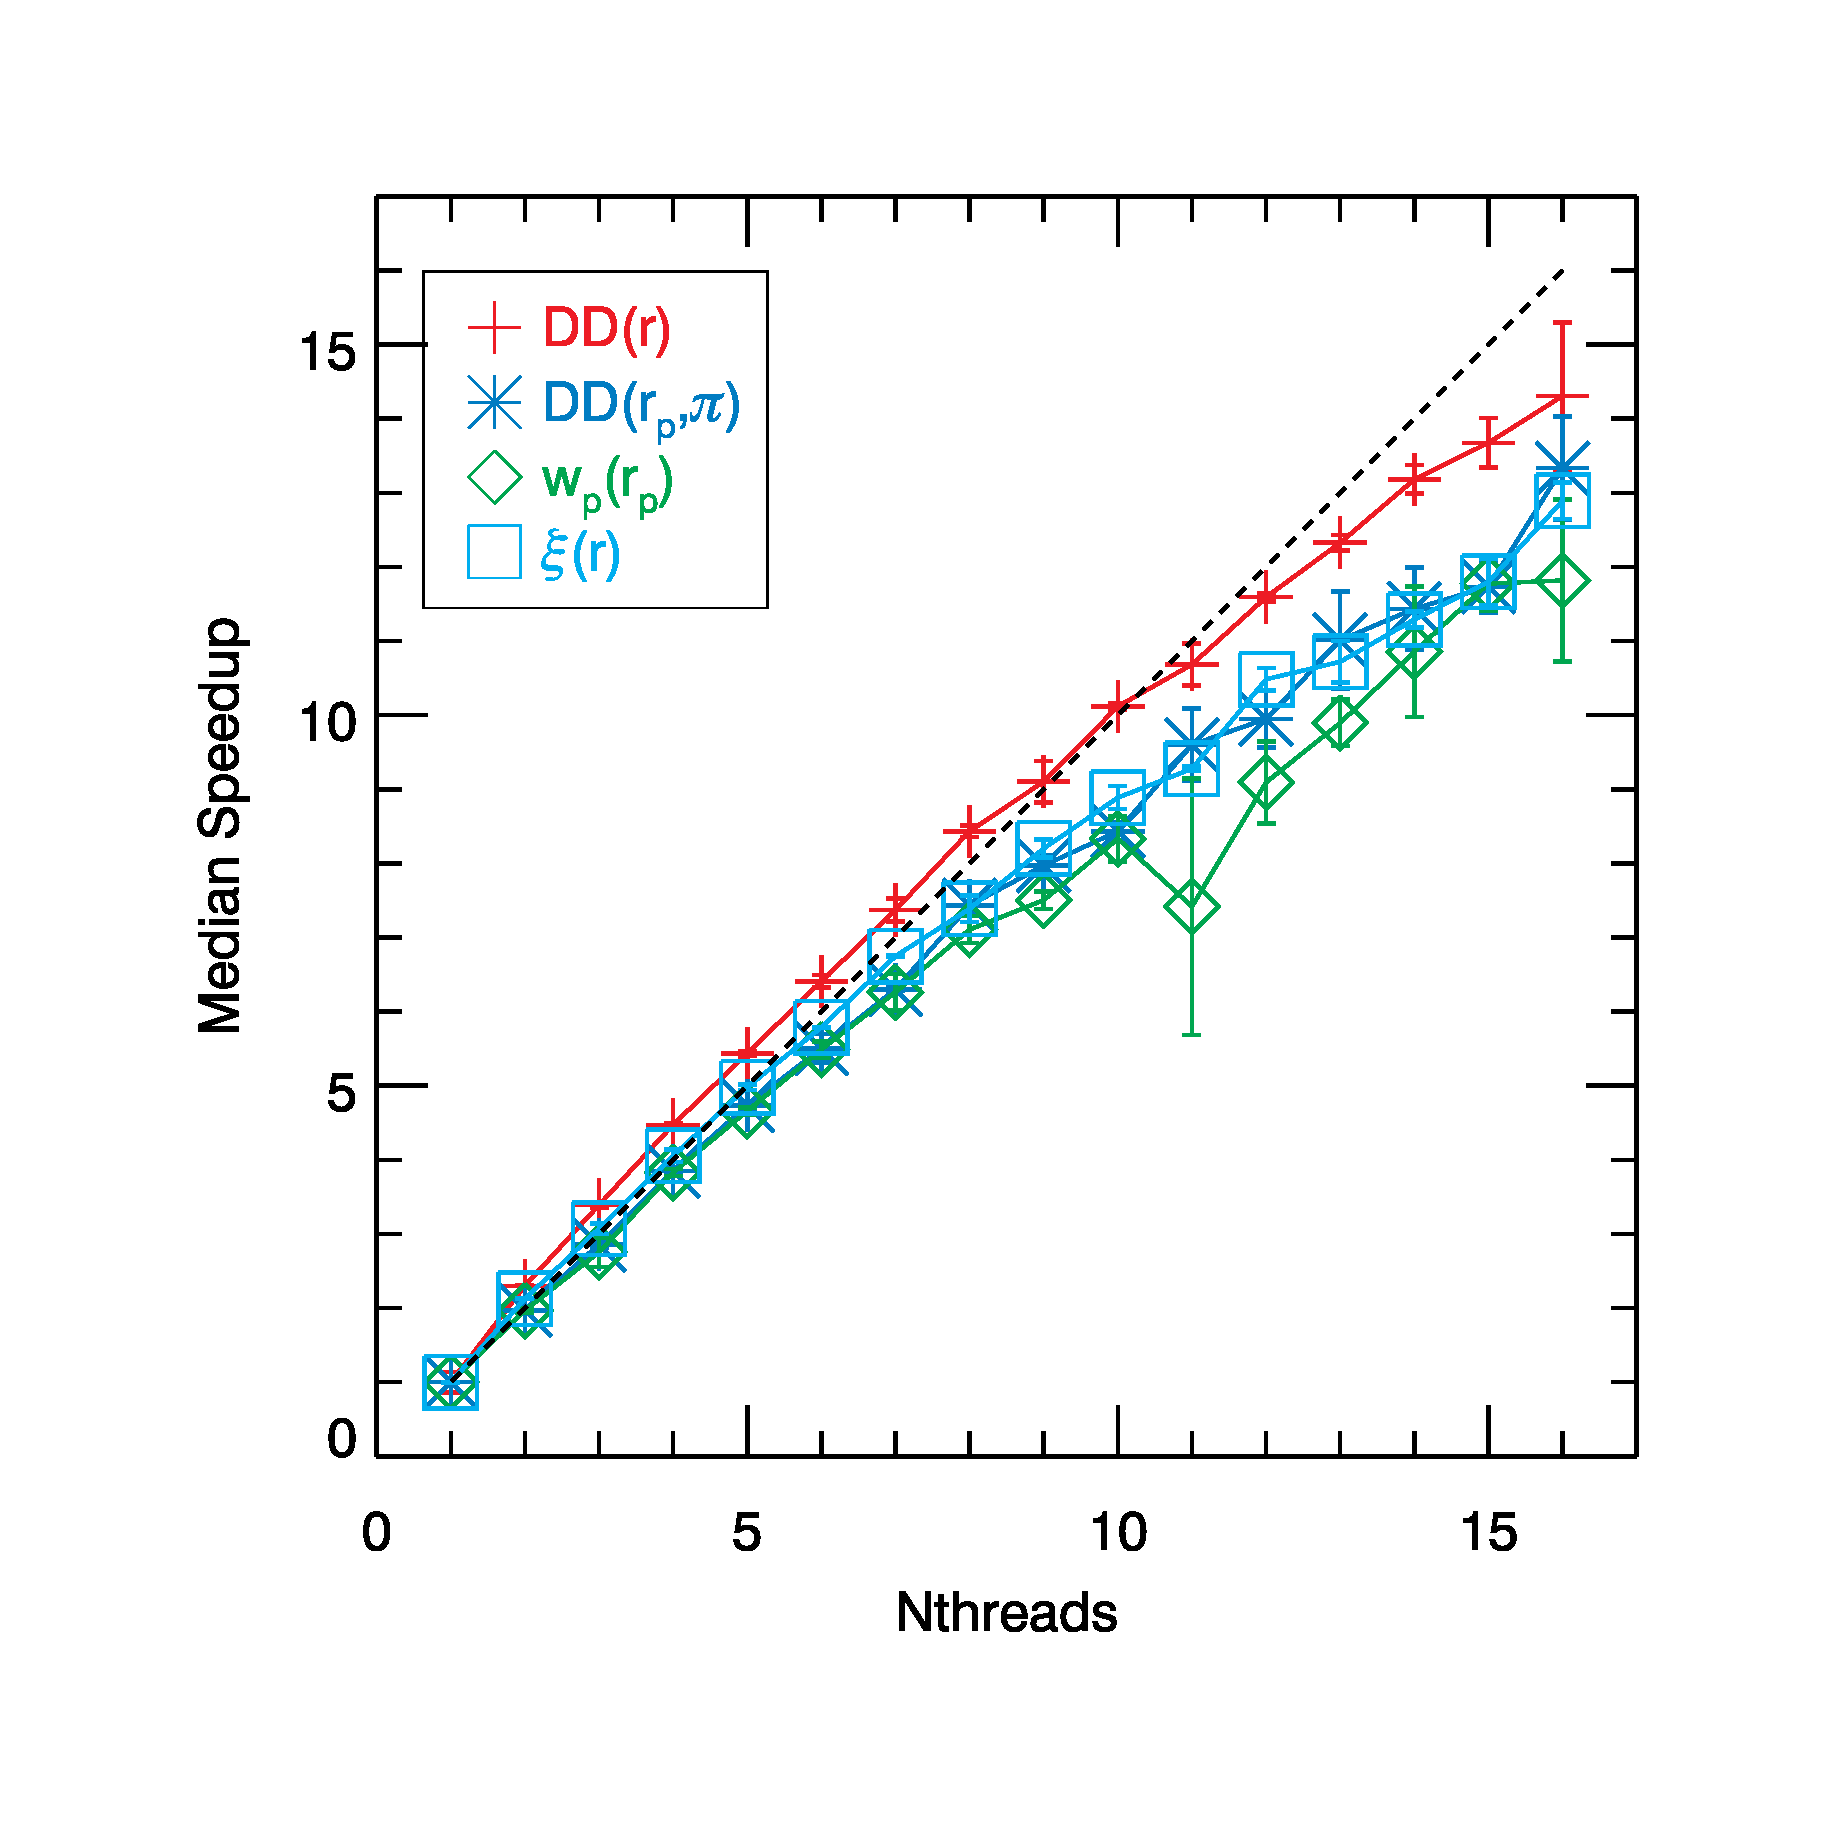
\includegraphics[clip=true,width=0.5\linewidth]{timings_Mr19_openmp}%
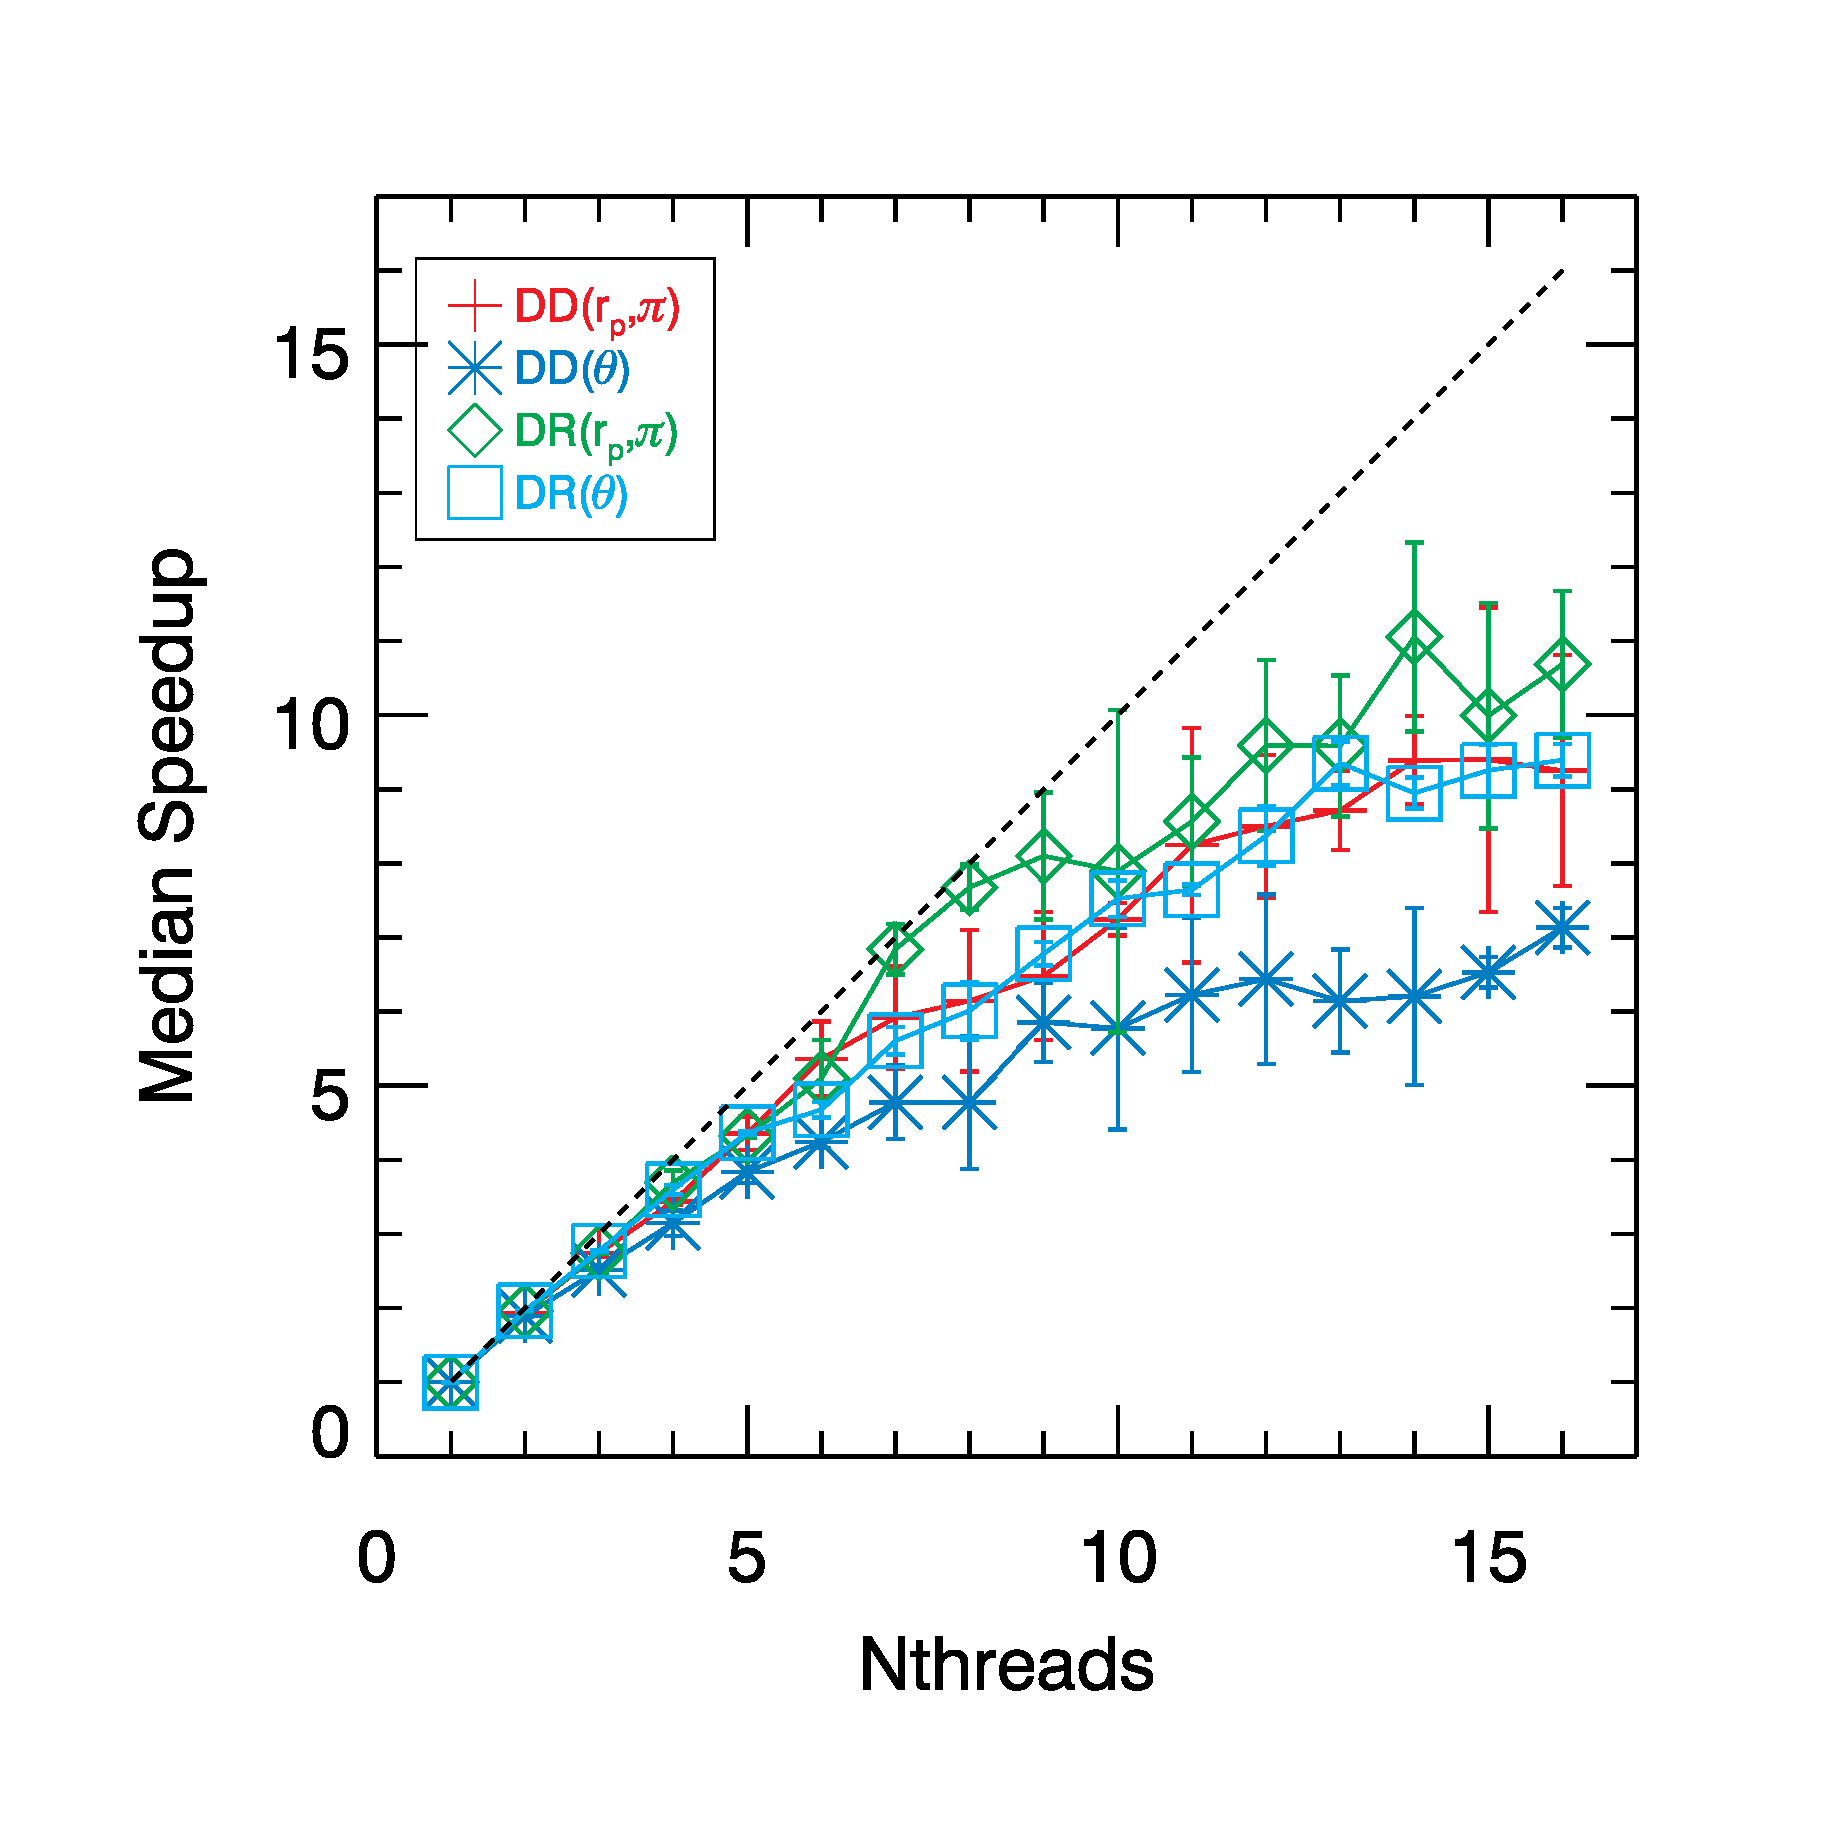
\includegraphics[clip=true,width=0.5\linewidth]{timings_Mr19_mocks_openmp}
\caption{OpenMP scaling for \xir, \xirppi, \wprp and \xiofr}
\label{fig:scaling_openmp}
\end{figure}

\begin{table}
\centering
\caption{\footnotesize OpenMP scaling for the three codes. Efficiencies are defined 
as \texttt{Speedup/Nthreads}. Note, that \xir has super-linear scaling with \texttt{nthreads}
up to $\sim$ 10 threads.}
\begin{adjustbox}{max width=\textwidth}
\begin{tabular}{ccccccccc} 
\toprule
\multirow{3}{*}{\textbf{Nthreads}}   &
\multicolumn{8}{c}{\textbf{Efficiency[\%]}} \\
\cmidrule(l{3em}r{3em}){2-9}

                                     &
\multicolumn{4}{c}{\textbf{Periodic Boxes}}  &
\multicolumn{4}{c}{\textbf{Spherical Geometry}}  \\
\cmidrule(l{1.0em}r{1.0em}){2-5}
\cmidrule(l{1.0em}r{1.0em}){6-9}
                                               &
\multicolumn{1}{c}{$\boldsymbol{\xir}$}        &
\multicolumn{1}{c}{$\boldsymbol{\xirppi}$}     &
\multicolumn{1}{c}{$\boldsymbol{\wprp}$}       & 
\multicolumn{1}{c}{$\boldsymbol{\xiofr}$}      &
\multicolumn{1}{c}{$\boldsymbol{DD(r_p,\pi)}$} &
\multicolumn{1}{c}{$\boldsymbol{DD(\theta)}$}  &
\multicolumn{1}{c}{$\boldsymbol{DR(r_p,\pi)}$} & 
\multicolumn{1}{c}{$\boldsymbol{DR(\theta)}$}   \\
\midrule
         1  &          100  &          100  &          100  &          100 &          100  &          100  &          100  &          100 \\
         2  &          115  &           98  &           98  &          106 &           96  &           94  &           97  &           98 \\
         3  &          113  &           95  &           91  &          102 &           91  &           83  &           91  &           92 \\
         4  &          111  &           96  &           95  &          101 &           85  &           78  &           92  &           89 \\
         5  &          108  &           94  &           93  &           99 &           87  &           76  &           86  &           87 \\
         6  &          106  &           91  &           91  &           96 &           89  &           70  &           84  &           77 \\
         7  &          105  &           90  &           89  &           96 &           84  &           68  &           97  &           80 \\
         8  &          105  &           92  &           88  &           92 &           76  &           59  &           95  &           75 \\
         9  &          101  &           88  &           83  &           91 &           72  &           65  &           89  &           75 \\
        10  &          101  &           84  &           83  &           88 &           72  &           57  &           78  &           75 \\
        11  &           97  &           87  &           67  &           84 &           74  &           56  &           77  &           69 \\
        12  &           96  &           82  &           75  &           87 &           70  &           53  &           79  &           69 \\
        13  &           94  &           84  &           76  &           82 &           67  &           47  &           73  &           71 \\
        14  &           94  &           81  &           77  &           80 &           67  &           44  &           78  &           63 \\
        15  &           91  &           78  &           78  &           78 &           62  &           43  &           66  &           61 \\
        16  &           89  &           83  &           73  &           80 &           57  &           44  &           66  &           58 \\

\bottomrule
\end{tabular}
\end{adjustbox}
\label{table:openmp}
\end{table}

\subsection{Speedup from SIMD code}

\begin{figure}[htbp]
\centering
\includegraphics[clip=true,scale=0.7]{wp_speedup_AVX}%
\caption{Speedup from AVX}
\label{fig:speedup_avx}
\end{figure}
\begin{figure}[htbp]
\centering
\includegraphics[clip=true,scale=0.7]{wp_speedup_SSE_4_2}
\caption{Speedup from AVX}
\label{fig:speedup_sse}
\end{figure}




\section{Conclusions}
I have presented a suite of three fast correlation function codes that take advantage of the underlying hardware. The reasons why the codes 
are much faster for typical workloads are:
\begin{itemize}
\item A `bin-lattice' scheme is used to first partition the computational domain into 3-D cells that can then be used to prune majority of the volume. 
\item To obtain better cache-locality, the particle list is duplicated into a contiguous array for each dimension. Thus, all particles that fall into the
same 3-D cell are stored in a contiguous array. 
\item With the AVX instruction set, modern CPU's can process 8 floats/4 doubles simultaneously. The codes contain hand-written AVX intrinsics that offer a 
factor of few speedup compared to the compiler generated scalar code. 
\end{itemize}
\citet{foreman-mackey_etal_13}

\section*{Acknowledgements}

\bibliographystyle{elsarticle-harv}
\bibliography{master}

\end{document}





%%% Local Variables:
%%% mode: latex
%%% TeX-master: t
%%% End:
